% ============================================================================
% NOAA Global Workflow Experiment Configuration System
% A Comprehensive Technical Reference
% ============================================================================
% Author: EIB MCP-RAG Development Team
% Date: February 11, 2026
% Version: 1.0
% ============================================================================

\documentclass[11pt,letterpaper]{article}

% ============================================================================
% PACKAGES
% ============================================================================

% Page layout
\usepackage[margin=1in]{geometry}
\usepackage{fancyhdr}

% Typography and fonts
\usepackage[T1]{fontenc}
\usepackage{lmodern}
\usepackage{microtype}

% Colors and graphics
\usepackage[dvipsnames,svgnames,table]{xcolor}
\usepackage{graphicx}
\usepackage{tikz}
\usetikzlibrary{shapes.geometric, arrows, positioning, fit, backgrounds, calc, decorations.pathreplacing}

% Tables
\usepackage{booktabs}
\usepackage{longtable}
\usepackage{array}

% Code listings
\usepackage{listings}
\usepackage{textcomp}

% Hyperlinks and PDF metadata
\usepackage[bookmarks=true,colorlinks=true,linkcolor=NavyBlue,urlcolor=NavyBlue,citecolor=NavyBlue]{hyperref}

% Math
\usepackage{amsmath}
\usepackage{amssymb}

% Misc
\usepackage{enumitem}
\usepackage{float}
\usepackage{caption}
\usepackage{subcaption}

% ============================================================================
% CUSTOM COLORS
% ============================================================================

\definecolor{NOAABlue}{RGB}{0, 51, 102}
\definecolor{NOAALightBlue}{RGB}{0, 102, 153}
\definecolor{CodeBackground}{RGB}{248, 248, 248}
\definecolor{CodeBorder}{RGB}{200, 200, 200}
\definecolor{CommentGreen}{RGB}{0, 128, 0}
\definecolor{StringOrange}{RGB}{206, 92, 0}
\definecolor{KeywordBlue}{RGB}{0, 0, 180}

% ============================================================================
% CODE LISTING STYLES
% ============================================================================

\lstdefinestyle{bashstyle}{
    language=bash,
    basicstyle=\ttfamily\small,
    backgroundcolor=\color{CodeBackground},
    frame=single,
    framerule=0.5pt,
    rulecolor=\color{CodeBorder},
    breaklines=true,
    breakatwhitespace=true,
    showstringspaces=false,
    numbers=left,
    numberstyle=\tiny\color{gray},
    numbersep=8pt,
    tabsize=2,
    keywordstyle=\color{KeywordBlue}\bfseries,
    commentstyle=\color{CommentGreen}\itshape,
    stringstyle=\color{StringOrange},
    morekeywords={export,source,if,then,else,fi,for,do,done,case,esac,function},
    literate={~}{{\textasciitilde}}1
             {>}{{\textgreater}}1
             {<}{{\textless}}1
}

\lstdefinestyle{pythonstyle}{
    language=Python,
    basicstyle=\ttfamily\small,
    backgroundcolor=\color{CodeBackground},
    frame=single,
    framerule=0.5pt,
    rulecolor=\color{CodeBorder},
    breaklines=true,
    breakatwhitespace=true,
    showstringspaces=false,
    numbers=left,
    numberstyle=\tiny\color{gray},
    numbersep=8pt,
    tabsize=4,
    keywordstyle=\color{KeywordBlue}\bfseries,
    commentstyle=\color{CommentGreen}\itshape,
    stringstyle=\color{StringOrange},
}

\lstdefinestyle{yamlstyle}{
    basicstyle=\ttfamily\small,
    backgroundcolor=\color{CodeBackground},
    frame=single,
    framerule=0.5pt,
    rulecolor=\color{CodeBorder},
    breaklines=true,
    showstringspaces=false,
    numbers=left,
    numberstyle=\tiny\color{gray},
    numbersep=8pt,
    tabsize=2,
    keywordstyle=\color{KeywordBlue}\bfseries,
    commentstyle=\color{CommentGreen}\itshape,
    stringstyle=\color{StringOrange},
    morestring=[b]",
    morestring=[b]',
    morecomment=[l]{\#},
    morekeywords={experiment,workflow,net,mode,pslot,app,resdetatmos,idate,edate,yaml,engine,rocoto},
}

\lstdefinestyle{xmlstyle}{
    language=XML,
    basicstyle=\ttfamily\small,
    backgroundcolor=\color{CodeBackground},
    frame=single,
    framerule=0.5pt,
    rulecolor=\color{CodeBorder},
    breaklines=true,
    showstringspaces=false,
    numbers=left,
    numberstyle=\tiny\color{gray},
    numbersep=8pt,
    tabsize=2,
}

% ============================================================================
% HEADER/FOOTER
% ============================================================================

\pagestyle{fancy}
\fancyhf{}
\fancyhead[L]{\small\textcolor{NOAABlue}{NOAA Global Workflow}}
\fancyhead[R]{\small\textcolor{NOAABlue}{Experiment Configuration System}}
\fancyfoot[C]{\thepage}
\renewcommand{\headrulewidth}{0.4pt}
\renewcommand{\footrulewidth}{0.4pt}

% ============================================================================
% TITLE PAGE INFO
% ============================================================================

\title{
    \vspace{-1cm}
    {\color{NOAABlue}\rule{\linewidth}{2pt}}\\[0.4cm]
    {\Huge\bfseries\color{NOAABlue} NOAA Global Workflow\\[0.3cm]
    Experiment Configuration System}\\[0.3cm]
    {\Large A Comprehensive Technical Reference}\\[0.2cm]
    {\color{NOAABlue}\rule{\linewidth}{2pt}}
}

\author{
    \textbf{Environmental Modeling Center}\\
    National Centers for Environmental Prediction\\
    NOAA/NWS\\[0.3cm]
    \textit{EIB MCP-RAG Development Team}
}

\date{February 11, 2026\\Version 1.0}

% ============================================================================
% DOCUMENT
% ============================================================================

\begin{document}

\maketitle
\thispagestyle{empty}

% ============================================================================
% EXECUTIVE SUMMARY
% ============================================================================

\begin{abstract}
\noindent
This document provides a comprehensive technical reference for the NOAA Global Workflow experiment configuration system. It details the complete lifecycle of experiment creation, from initial definition through YAML case files or command-line interface, through Jinja2 template rendering, to runtime configuration sourcing during job execution on High Performance Computing (HPC) platforms.

The document covers the application factory pattern used to register six distinct application types (GFS, GEFS, SFS, GCAFS in cycled and forecast-only modes), the hierarchical configuration file system with 105+ config files including 16 Jinja2 templates, platform-specific resource allocation for seven HPC platforms, and the Rocoto workflow engine integration.

This reference is intended for developers, operators, system administrators, and stakeholders seeking to understand the internal architecture of the Global Workflow experiment configuration system.
\end{abstract}

\newpage
\tableofcontents
\newpage

% ============================================================================
% SECTION 1: INTRODUCTION
% ============================================================================

\section{Introduction}

\subsection{Purpose and Scope}

The NOAA Global Workflow is the operational infrastructure for numerical weather prediction (NWP) at the National Centers for Environmental Prediction (NCEP). This system produces the Global Forecast System (GFS) and related ensemble and coupled model forecasts that support weather prediction worldwide.

This document provides a complete technical reference for understanding how experiments are configured and instantiated within the Global Workflow. An \textbf{experiment} in this context refers to a specific configuration of the workflow for a particular purpose, such as:

\begin{itemize}
    \item Operational production forecasts
    \item Development and testing
    \item Continuous integration validation
    \item Retrospective analyses
    \item Research experiments
\end{itemize}

\subsection{Target Audience}

This document is intended for:

\begin{description}
    \item[Developers] Writing new components or modifying existing workflow functionality
    \item[Operators] Running and monitoring workflow experiments on HPC systems
    \item[System Administrators] Managing infrastructure and resource allocation
    \item[New Team Members] Onboarding to understand the system architecture
    \item[Stakeholders] Requiring technical understanding of the system
\end{description}

\subsection{Document Conventions}

\begin{itemize}
    \item \texttt{Monospace text} indicates file names, paths, commands, or code
    \item \textbf{Bold text} indicates important terms or emphasis
    \item \textcolor{NOAABlue}{Blue text} indicates hyperlinks
    \item Code blocks include syntax highlighting for clarity
    \item Diagrams use consistent color coding: blue for Python, orange for Bash, green for YAML
\end{itemize}

\subsection{System Overview}

The Global Workflow experiment configuration system operates through three distinct phases:

\begin{enumerate}
    \item \textbf{Experiment Definition} --- Specification of parameters via YAML or CLI
    \item \textbf{Experiment Setup} --- Directory creation and template rendering
    \item \textbf{Runtime Configuration} --- Dynamic sourcing during job execution
\end{enumerate}

Figure \ref{fig:high-level-overview} illustrates this three-phase architecture.

\begin{figure}[H]
\centering
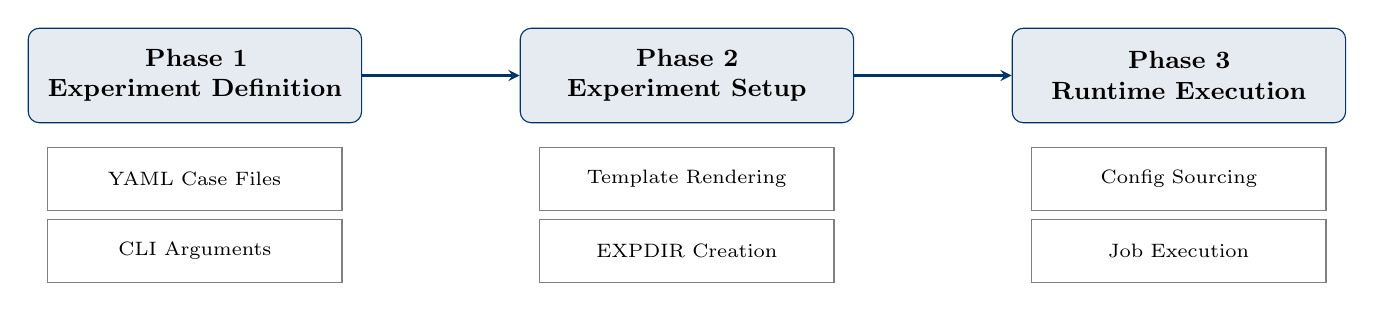
\begin{tikzpicture}[
    node distance=0.8cm,
    phase/.style={rectangle, rounded corners, draw=NOAABlue, fill=NOAABlue!10, 
                  text width=4cm, minimum height=1.2cm, align=center, font=\small\bfseries},
    component/.style={rectangle, draw=gray, fill=white, 
                      text width=3.5cm, minimum height=0.8cm, align=center, font=\scriptsize},
    arrow/.style={->, thick, >=stealth, color=NOAABlue}
]

% Phase 1
\node[phase] (p1) {Phase 1\\Experiment Definition};
\node[component, below=0.3cm of p1] (yaml) {YAML Case Files};
\node[component, below=0.1cm of yaml] (cli) {CLI Arguments};

% Phase 2
\node[phase, right=2cm of p1] (p2) {Phase 2\\Experiment Setup};
\node[component, below=0.3cm of p2] (render) {Template Rendering};
\node[component, below=0.1cm of render] (expdir) {EXPDIR Creation};

% Phase 3
\node[phase, right=2cm of p2] (p3) {Phase 3\\Runtime Execution};
\node[component, below=0.3cm of p3] (source) {Config Sourcing};
\node[component, below=0.1cm of source] (jobs) {Job Execution};

% Arrows
\draw[arrow] (p1) -- (p2);
\draw[arrow] (p2) -- (p3);

\end{tikzpicture}
\caption{High-Level Overview of Experiment Configuration Phases}
\label{fig:high-level-overview}
\end{figure}

% ============================================================================
% SECTION 2: SYSTEM ARCHITECTURE
% ============================================================================

\section{System Architecture Overview}

\subsection{Directory Structure}

The Global Workflow follows a standardized directory structure organized by function:

\begin{lstlisting}[style=bashstyle, title=Global Workflow Directory Structure]
global-workflow/
├── dev/                    # Development directory
│   ├── ci/                 # Continuous integration
│   │   └── cases/          # YAML case files for CI testing
│   ├── jobs/               # J-job scripts (entry points)
│   ├── parm/               # Parameter and config files
│   │   └── config/         # Configuration by network (gfs, gcafs, etc.)
│   └── workflow/           # Python workflow infrastructure
│       ├── applications/   # Application factory
│       └── rocoto/         # Rocoto workflow generation
├── scripts/                # Execution scripts (ex*.sh)
├── ush/                    # Utility scripts
├── env/                    # Platform environment files
├── parm/                   # Shared parameter files
└── sorc/                   # Source code and build
\end{lstlisting}

\subsection{Component Relationships}

Figure \ref{fig:component-diagram} shows the relationships between major system components.

\begin{figure}[H]
\centering
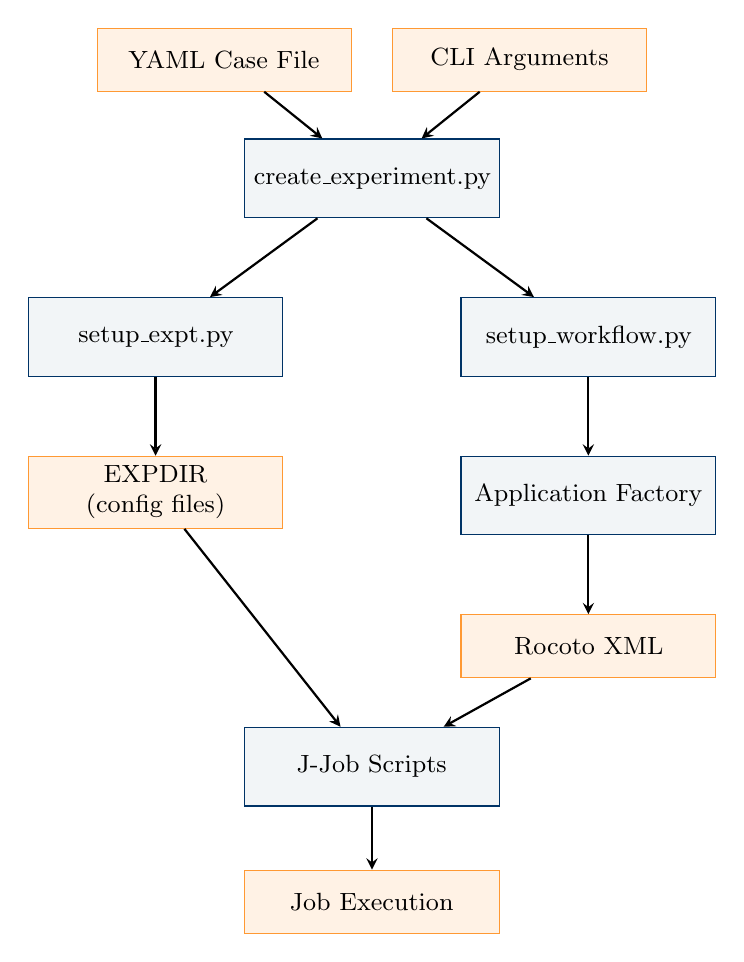
\begin{tikzpicture}[
    node distance=1cm,
    box/.style={rectangle, draw=NOAABlue, fill=NOAABlue!5, 
                text width=3cm, minimum height=1cm, align=center, font=\small},
    databox/.style={rectangle, draw=orange!80, fill=orange!10, 
                    text width=3cm, minimum height=0.8cm, align=center, font=\small},
    arrow/.style={->, thick, >=stealth},
    darrow/.style={<->, thick, >=stealth, color=gray}
]

% User inputs
\node[databox] (yaml) {YAML Case File};
\node[databox, right=0.5cm of yaml] (cli) {CLI Arguments};

% Setup scripts
\node[box, below=1cm of $(yaml)!0.5!(cli)$] (create) {create\_experiment.py};
\node[box, below left=1cm and -0.5cm of create] (setup_expt) {setup\_expt.py};
\node[box, below right=1cm and -0.5cm of create] (setup_wf) {setup\_workflow.py};

% Application factory
\node[box, below=1cm of setup_wf] (factory) {Application Factory};

% Outputs
\node[databox, below=1cm of setup_expt] (expdir) {EXPDIR\\(config files)};
\node[databox, below=1cm of factory] (xml) {Rocoto XML};

% Runtime
\node[box, below=2cm of $(expdir)!0.5!(xml)$] (jjob) {J-Job Scripts};
\node[databox, below=0.8cm of jjob] (exec) {Job Execution};

% Arrows
\draw[arrow] (yaml) -- (create);
\draw[arrow] (cli) -- (create);
\draw[arrow] (create) -- (setup_expt);
\draw[arrow] (create) -- (setup_wf);
\draw[arrow] (setup_expt) -- (expdir);
\draw[arrow] (setup_wf) -- (factory);
\draw[arrow] (factory) -- (xml);
\draw[arrow] (expdir) -- (jjob);
\draw[arrow] (xml) -- (jjob);
\draw[arrow] (jjob) -- (exec);

\end{tikzpicture}
\caption{Component Relationship Diagram}
\label{fig:component-diagram}
\end{figure}

\subsection{Data Flow Overview}

\begin{enumerate}
    \item \textbf{Input}: User provides experiment specification (YAML or CLI)
    \item \textbf{Processing}: Python scripts create directories and render templates
    \item \textbf{Generation}: Application factory produces Rocoto workflow XML
    \item \textbf{Execution}: Rocoto orchestrates job submission and dependency management
    \item \textbf{Runtime}: J-jobs source configuration and execute scripts
\end{enumerate}

% ============================================================================
% SECTION 3: APPLICATION FACTORY PATTERN
% ============================================================================

\section{Application Factory Pattern}

\subsection{Design Pattern Overview}

The Global Workflow uses the \textbf{Factory Pattern} to instantiate application configurations dynamically based on the network type (NET) and operational mode (MODE). This design enables:

\begin{itemize}
    \item \textbf{Extensibility}: New application types can be added without modifying core logic
    \item \textbf{Encapsulation}: Each application manages its own task definitions
    \item \textbf{Consistency}: Uniform interface across all application types
\end{itemize}

\subsection{Registered Applications}

The factory registers six application configurations:

\begin{table}[H]
\centering
\caption{Registered Application Configurations}
\label{tab:applications}
\begin{tabular}{@{}llll@{}}
\toprule
\textbf{Registration Key} & \textbf{NET} & \textbf{MODE} & \textbf{Class} \\
\midrule
\texttt{gfs\_cycled} & GFS & Cycled & GFSCycledAppConfig \\
\texttt{gfs\_forecast-only} & GFS & Forecast-only & GFSForecastOnlyAppConfig \\
\texttt{gefs\_forecast-only} & GEFS & Forecast-only & GEFSAppConfig \\
\texttt{sfs\_forecast-only} & SFS & Forecast-only & SFSAppConfig \\
\texttt{gcafs\_forecast-only} & GCAFS & Forecast-only & GCAFSForecastOnlyAppConfig \\
\texttt{gcafs\_cycled} & GCAFS & Cycled & GCAFSCycledAppConfig \\
\bottomrule
\end{tabular}
\end{table}

\subsection{Factory Implementation}

\begin{lstlisting}[style=pythonstyle, title=application\_factory.py]
from wxflow import Factory
from applications.gfs_cycled import GFSCycledAppConfig
from applications.gfs_forecast_only import GFSForecastOnlyAppConfig
from applications.gefs import GEFSAppConfig
from applications.sfs import SFSAppConfig
from applications.gcafs_forecast_only import GCAFSForecastOnlyAppConfig
from applications.gcafs_cycled import GCAFSCycledAppConfig

# Initialize the application configuration factory
app_config_factory = Factory('AppConfig')

# Register application configurations
app_config_factory.register('gfs_cycled', GFSCycledAppConfig)
app_config_factory.register('gfs_forecast-only', GFSForecastOnlyAppConfig)
app_config_factory.register('gefs_forecast-only', GEFSAppConfig)
app_config_factory.register('sfs_forecast-only', SFSAppConfig)
app_config_factory.register('gcafs_forecast-only', GCAFSForecastOnlyAppConfig)
app_config_factory.register('gcafs_cycled', GCAFSCycledAppConfig)
\end{lstlisting}

\subsection{AppConfig Base Class}

All application configurations inherit from the \texttt{AppConfig} base class, which defines the interface for task generation:

\begin{lstlisting}[style=pythonstyle, title=applications.py (Base Class)]
from abc import ABC, abstractmethod

class AppConfig(ABC):
    """Base configuration class for all applications."""
    
    def __init__(self, conf):
        self.conf = conf
        self._base = conf.parse_config('config.base')
    
    @abstractmethod
    def get_task_names(self) -> dict:
        """Return dictionary of task names by run type.
        
        Returns
        -------
        dict
            Keys are run types (e.g., 'gfs', 'gdas')
            Values are lists of task names in execution order
        """
        pass
\end{lstlisting}

\subsection{Task Name Generation Example}

Each application defines its tasks and their order:

\begin{lstlisting}[style=pythonstyle, title=gfs\_cycled.py (Excerpt)]
class GFSCycledAppConfig(AppConfig):
    
    def get_task_names(self) -> dict:
        task_names = {
            'gdas': ['prep', 'anal', 'sfcanl', 'analcalc', 
                     'fcst', 'upp', 'atmos_products'],
            'gfs':  ['fetch', 'prep', 'atmanlinit', 'atmanlvar',
                     'atmanlfv3inc', 'atmanlfinal', 'sfcanl',
                     'analcalc', 'fcst', 'upp', 'atmos_products',
                     'tracker', 'genesis', 'arch']
        }
        
        # Add optional tasks based on configuration
        if self._base.get('DO_WAVE', 'NO') == 'YES':
            for run in task_names:
                task_names[run].extend(['waveinit', 'waveprep',
                                        'wavepostsbs', 'wavepostpnt'])
        
        return task_names
\end{lstlisting}

% ============================================================================
% SECTION 4: EXPERIMENT DEFINITION
% ============================================================================

\section{Experiment Definition}

\subsection{Two Methods of Experiment Definition}

Experiments can be defined through two equivalent methods:

\begin{table}[H]
\centering
\caption{Experiment Definition Methods}
\label{tab:definition-methods}
\begin{tabular}{@{}lll@{}}
\toprule
\textbf{Method} & \textbf{Use Case} & \textbf{Entry Point} \\
\midrule
YAML Case File & CI testing, reproducible configs & \texttt{create\_experiment.py -y file.yaml} \\
CLI Arguments & Interactive/manual setup & \texttt{setup\_expt.py NET MODE --args} \\
\bottomrule
\end{tabular}
\end{table}

\subsection{YAML Case File Structure}

YAML case files provide a complete experiment specification:

\begin{lstlisting}[style=yamlstyle, title=Example: C48\_S2SW.yaml]
experiment:
  net: gfs
  mode: forecast-only
  pslot: {{ 'pslot' | getenv }}
  app: S2SW
  resdetatmos: 48
  resdetocean: 5.0
  comroot: {{ 'RUNTESTS' | getenv }}/COMROOT
  expdir: {{ 'RUNTESTS' | getenv }}/EXPDIR
  idate: 2021032312
  edate: 2021032312
  yaml: {{ HOMEgfs }}/dev/ci/cases/yamls/gfs_defaults_ci.yaml

workflow:
  engine: rocoto
  rocoto:
    maxtries: 2
    cyclethrottle: 3
    taskthrottle: 25
    verbosity: 2
\end{lstlisting}

\subsection{Key Experiment Parameters}

\begin{table}[H]
\centering
\caption{Experiment Definition Parameters}
\label{tab:exp-params}
\begin{tabular}{@{}llp{6cm}@{}}
\toprule
\textbf{Parameter} & \textbf{Example} & \textbf{Description} \\
\midrule
\texttt{net} & \texttt{gfs} & Network type (gfs, gefs, gcafs, sfs) \\
\texttt{mode} & \texttt{cycled} & Operational mode (cycled, forecast-only) \\
\texttt{pslot} & \texttt{C384\_S2SW} & Experiment slot name \\
\texttt{app} & \texttt{S2SW} & Application type (ATM, S2S, S2SW, S2SWA) \\
\texttt{resdetatmos} & \texttt{384} & Atmospheric resolution (becomes C384) \\
\texttt{resdetocean} & \texttt{0.25} & Ocean resolution (becomes 025) \\
\texttt{idate} & \texttt{2021032312} & Initial date (YYYYMMDDHH) \\
\texttt{edate} & \texttt{2021033112} & End date (YYYYMMDDHH) \\
\texttt{nens} & \texttt{20} & Number of ensemble members \\
\texttt{start} & \texttt{cold} & Start type (cold, warm) \\
\bottomrule
\end{tabular}
\end{table}

\subsection{CLI-Based Experiment Setup}

\begin{lstlisting}[style=bashstyle, title=CLI Experiment Setup]
# GFS Cycled experiment
python setup_expt.py gfs cycled \
    --pslot C384_S2SW \
    --app S2SW \
    --resdetatmos 384 \
    --resdetocean 0.25 \
    --idate 2024010100 \
    --edate 2024011000 \
    --expdir /scratch/expdir \
    --comroot /scratch/comroot

# GEFS Forecast-only experiment
python setup_expt.py gefs forecast-only \
    --pslot C384_GEFS_20mem \
    --nens 20 \
    --resdetatmos 384 \
    --idate 2024010100
\end{lstlisting}

\subsection{CI Case File Categories}

The CI system organizes case files by purpose:

\begin{table}[H]
\centering
\caption{CI Case File Categories}
\label{tab:ci-cases}
\begin{tabular}{@{}llp{5.5cm}@{}}
\toprule
\textbf{Directory} & \textbf{Count} & \textbf{Purpose} \\
\midrule
\texttt{pr/} & 20 & Pull request tests (run on every PR) \\
\texttt{gfsv17/} & 20 & GFS v17 production-like configurations \\
\texttt{gcafsv1/} & 6 & GCAFS v1 tests \\
\texttt{sfsv1/} & 2 & SFS v1 tests \\
\texttt{hires/} & 2 & High-resolution tests (C768, C1152) \\
\texttt{weekly/} & 2 & Weekly extended tests \\
\texttt{yamls/} & 19 & Default settings (included by cases) \\
\bottomrule
\end{tabular}
\end{table}

% ============================================================================
% SECTION 5: CONFIGURATION FILE SYSTEM
% ============================================================================

\section{Configuration File System}

\subsection{Configuration File Categories}

The GFS configuration directory contains 105 files organized into categories:

\begin{table}[H]
\centering
\caption{Configuration File Statistics}
\label{tab:config-stats}
\begin{tabular}{@{}lr@{}}
\toprule
\textbf{Category} & \textbf{Count} \\
\midrule
Jinja2 Templates (\texttt{*.j2}) & 16 \\
Plain Bash Configs & 88 \\
YAML Defaults Directory & 1 \\
\midrule
\textbf{Total} & 105 \\
\bottomrule
\end{tabular}
\end{table}

\subsection{Jinja2 Template Files}

Templates are rendered at setup time with experiment-specific values:

\begin{table}[H]
\centering
\caption{Jinja2 Template Files}
\label{tab:j2-templates}
\begin{tabular}{@{}lp{7cm}@{}}
\toprule
\textbf{Template} & \textbf{Purpose} \\
\midrule
\texttt{config.base.j2} & Global settings (machine, paths, toggles) \\
\texttt{config.fcst.j2} & Forecast configuration \\
\texttt{config.atmanl.j2} & Atmospheric analysis \\
\texttt{config.atmensanl.j2} & Ensemble atmospheric analysis \\
\texttt{config.marineanl.j2} & Marine analysis \\
\texttt{config.marinebmat.j2} & Marine background error matrix \\
\texttt{config.marineanlecen.j2} & Marine ensemble centering \\
\texttt{config.marineanlletkf.j2} & Marine LETKF analysis \\
\texttt{config.aeroanl.j2} & Aerosol analysis \\
\texttt{config.aero.j2} & Aerosol configuration \\
\texttt{config.prep.j2} & Data preparation \\
\texttt{config.prepoceanobs.j2} & Ocean observation preparation \\
\texttt{config.snowanl.j2} & Snow analysis \\
\texttt{config.esnowanl.j2} & Ensemble snow analysis \\
\texttt{config.ocn.j2} & Ocean configuration \\
\texttt{config.stage\_ic.j2} & Initial condition staging \\
\bottomrule
\end{tabular}
\end{table}

\subsection{Template Rendering Example}

\begin{lstlisting}[style=bashstyle, title=config.base.j2 Template (Excerpt)]
#! /usr/bin/env bash

########## config.base ##########
# Common to all steps

echo "BEGIN: config.base"

# Machine environment
export machine="{{ MACHINE }}"

# Account, queue, etc.
export ACCOUNT="{{ ACCOUNT }}"
export QUEUE="{{ QUEUE }}"
export PARTITION_BATCH="{{ PARTITION_BATCH }}"

# Experiment settings
export PSLOT="{{ PSLOT }}"
export CASE="{{ CASE_CTL }}"

# Directories
export HOMEgfs="{{ HOMEgfs }}"
export EXPDIR="{{ EXPDIR }}"
export COMROOT="{{ COMROOT }}"
\end{lstlisting}

After rendering with context \texttt{\{MACHINE: "HERA", PSLOT: "C384\_S2SW", CASE\_CTL: "C384"\}}:

\begin{lstlisting}[style=bashstyle, title=Rendered config.base]
#! /usr/bin/env bash

########## config.base ##########
# Common to all steps

echo "BEGIN: config.base"

# Machine environment
export machine="HERA"

# Account, queue, etc.
export ACCOUNT="da-cpu"
export QUEUE="batch"
export PARTITION_BATCH=""

# Experiment settings
export PSLOT="C384_S2SW"
export CASE="C384"

# Directories
export HOMEgfs="/home/user/global-workflow"
export EXPDIR="/scratch/expdir/C384_S2SW"
export COMROOT="/scratch/comroot"
\end{lstlisting}

\subsection{Hierarchical Config Structure}

Configuration files follow a hierarchical inheritance pattern:

\begin{figure}[H]
\centering
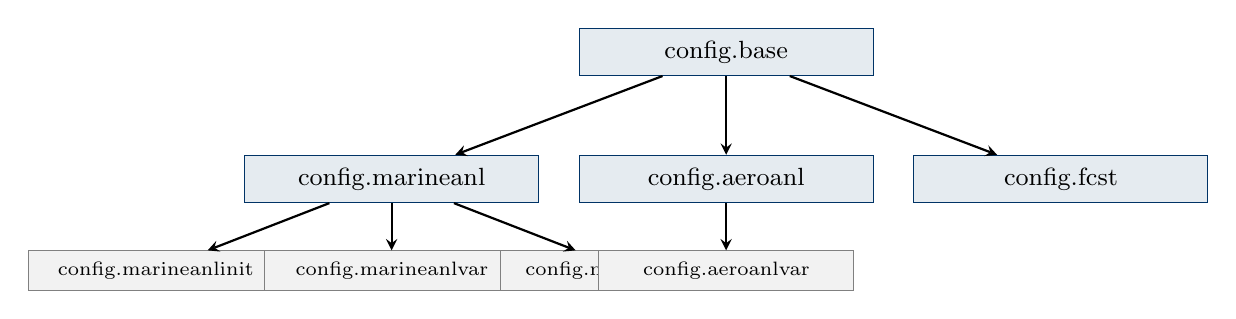
\begin{tikzpicture}[
    node distance=0.6cm,
    box/.style={rectangle, draw=NOAABlue, fill=NOAABlue!10, 
                text width=3.5cm, minimum height=0.6cm, align=center, font=\small},
    subbox/.style={rectangle, draw=gray, fill=gray!10, 
                   text width=3cm, minimum height=0.5cm, align=center, font=\scriptsize},
    arrow/.style={->, thick, >=stealth}
]

% Base
\node[box] (base) {config.base};

% Subsystems
\node[box, below left=1cm and 0.5cm of base] (marineanl) {config.marineanl};
\node[box, below=1cm of base] (aeroanl) {config.aeroanl};
\node[box, below right=1cm and 0.5cm of base] (fcst) {config.fcst};

% Sub-steps
\node[subbox, below left=0.6cm and -0.5cm of marineanl] (marineinit) {config.marineanlinit};
\node[subbox, below=0.6cm of marineanl] (marinevar) {config.marineanlvar};
\node[subbox, below right=0.6cm and -0.5cm of marineanl] (marinefinal) {config.marineanlfinal};

\node[subbox, below=0.6cm of aeroanl] (aerovar) {config.aeroanlvar};

% Arrows
\draw[arrow] (base) -- (marineanl);
\draw[arrow] (base) -- (aeroanl);
\draw[arrow] (base) -- (fcst);

\draw[arrow] (marineanl) -- (marineinit);
\draw[arrow] (marineanl) -- (marinevar);
\draw[arrow] (marineanl) -- (marinefinal);

\draw[arrow] (aeroanl) -- (aerovar);

\end{tikzpicture}
\caption{Hierarchical Configuration Inheritance}
\label{fig:config-hierarchy}
\end{figure}

% ============================================================================
% SECTION 6: PLATFORM RESOURCE CONFIGURATION
% ============================================================================

\section{Platform Resource Configuration}

\subsection{Three-Layer Resource Architecture}

Resource allocation follows a three-layer architecture that enables platform-independent experiment definitions while supporting platform-specific optimizations:

\begin{figure}[H]
\centering
\begin{tikzpicture}[
    node distance=0.8cm,
    layer/.style={rectangle, draw=NOAABlue, fill=NOAABlue!10, 
                  text width=10cm, minimum height=1.2cm, align=center, font=\small},
    arrow/.style={->, thick, >=stealth, color=NOAABlue}
]

\node[layer] (l3) {\textbf{Layer 3: Platform-Specific Overrides}\\
\texttt{config.resources.HERA}, \texttt{config.resources.WCOSS2}, etc.};

\node[layer, below=0.5cm of l3] (l2) {\textbf{Layer 2: Base Resource Definitions}\\
\texttt{config.resources} --- Default resources per task × CASE resolution};

\node[layer, below=0.5cm of l2] (l1) {\textbf{Layer 1: Experiment Setup}\\
CASE file or CLI sets \$CASE, \$machine, \$RUN};

\draw[arrow] (l1) -- (l2) node[midway, right, font=\scriptsize] {sources};
\draw[arrow] (l2) -- (l3) node[midway, right, font=\scriptsize] {sources};

\end{tikzpicture}
\caption{Three-Layer Resource Configuration Architecture}
\label{fig:resource-layers}
\end{figure}

\subsection{Platform Physical Limits}

Each HPC platform has fixed physical constraints:

\begin{table}[H]
\centering
\caption{HPC Platform Physical Limits}
\label{tab:platform-limits}
\begin{tabular}{@{}lrrl@{}}
\toprule
\textbf{Platform} & \textbf{Tasks/Node} & \textbf{Memory/Node} & \textbf{Notes} \\
\midrule
WCOSS2 & 128 & 500 GB & Production (reservable: 500GB) \\
HERA & 40 & 96 GB & R\&D primary \\
HERCULES & 80 & 500 GB & R\&D \\
ORION & 40 & 180 GB & R\&D \\
GAEA C5 & 128 & 251 GB & Climate R\&D \\
GAEA C6 & 192 & 384 GB & Climate R\&D \\
URSA & 192 & 360 GB & Cloud \\
\bottomrule
\end{tabular}
\end{table}

\subsection{Resource Definition by Task and Resolution}

The \texttt{config.resources} script computes resources based on task and CASE:

\begin{lstlisting}[style=bashstyle, title=config.resources (Excerpt)]
case ${step} in
  "anal")
    if [[ "${RUN}" = *gdas ]]; then
      walltime="01:20:00"
      case ${CASE} in
        "C1152" | "C768")
          ntasks=780
          threads_per_task=5
          walltime="01:40:00"
          ;;
        "C384" | "C192")
          ntasks=160
          threads_per_task=10
          ;;
        "C96" | "C48")
          ntasks=84
          threads_per_task=5
          ;;
      esac
    fi
    tasks_per_node=$(( max_tasks_per_node / threads_per_task ))
    is_exclusive=True
    ;;
esac
\end{lstlisting}

\subsection{Platform Override Example}

\begin{lstlisting}[style=bashstyle, title=config.resources.HERA]
case ${step} in
  "prep")
    # Run on fewer tasks per node for memory requirement
    tasks_per_node=2
    ;;
    
  "eupd")
    case "${CASE}" in
      "C384")
        export ntasks=80  # Hera-specific reduction
        ;;
    esac
    export tasks_per_node=$(( max_tasks_per_node / threads_per_task ))
    ;;
esac
\end{lstlisting}

\subsection{Complete Resource Matrix}

\begin{table}[H]
\centering
\caption{Resource Allocation by Task and Resolution (Selected Tasks)}
\label{tab:resource-matrix}
\small
\begin{tabular}{@{}llrrrr@{}}
\toprule
\textbf{Task} & \textbf{CASE} & \textbf{ntasks} & \textbf{threads} & \textbf{walltime} & \textbf{memory} \\
\midrule
anal & C768 & 780 & 5 & 01:40:00 & exclusive \\
anal & C384 & 160 & 10 & 01:20:00 & exclusive \\
anal & C96 & 84 & 5 & 01:20:00 & exclusive \\
\midrule
fcst (gfs) & C768 & varies & varies & 06:00:00 & exclusive \\
fcst (gfs) & C384 & varies & varies & 06:00:00 & exclusive \\
fcst (gdas) & C384 & varies & varies & 00:30:00 & exclusive \\
\midrule
upp & C1152 & 200 & 1 & 00:15:00 & max\_node \\
upp & C768 & 120 & 1 & 00:15:00 & max\_node \\
upp & C48 & 48 & 1 & 00:15:00 & --- \\
\midrule
eupd & C768 & 480 & 6 & 00:45:00 & exclusive \\
eupd & C384 & 270 & 8 & 00:45:00 & exclusive \\
\bottomrule
\end{tabular}
\end{table}

% ============================================================================
% SECTION 7: EXPERIMENT DIRECTORY POPULATION
% ============================================================================

\section{Experiment Directory Population}

\subsection{create\_experiment.py Workflow}

The \texttt{create\_experiment.py} script orchestrates the complete setup:

\begin{lstlisting}[style=pythonstyle, title=create\_experiment.py (Simplified)]
if __name__ == '__main__':
    user_inputs = input_args()
    
    # Parse YAML with Jinja2 templating
    data = AttrDict(HOMEgfs=_top)
    data.update(os.environ)
    testconf = parse_j2yaml(path=user_inputs.yaml, data=data)
    
    # Build arguments for setup_expt.py
    setup_expt_args = [testconf.experiment.net, 
                       testconf.experiment.mode]
    for kk, vv in testconf.experiment.items():
        if kk not in ['net', 'mode']:
            setup_expt_args.extend([f"--{kk}", str(vv)])
    
    # Run setup_expt.py
    setup_expt.main(setup_expt_args)
    
    # Run setup_workflow.py
    experiment_dir = Path(testconf.experiment.expdir) / \
                     Path(testconf.experiment.pslot)
    setup_workflow.main([str(experiment_dir), 'rocoto'])
\end{lstlisting}

\subsection{Template Rendering Process}

\begin{lstlisting}[style=pythonstyle, title=update\_configs() Function]
def update_configs(host, inputs):
    """Copy and render config files to EXPDIR."""
    
    # Combine host info and user inputs
    host_plus_inputs = AttrDict(host.info, **inputs_dict)
    host_plus_inputs.HOMEgfs = _top
    host_plus_inputs.MACHINE = str(host).upper()
    
    # Process each file in config directory
    files = os.listdir(inputs.configdir)
    for file in files:
        if file.endswith('.j2'):  # Jinja2 template
            input_template = f'{inputs.configdir}/{file}'
            output_file = f'{inputs.expdir}/{inputs.pslot}/{file[:-3]}'
            
            # Render template
            Jinja(input_template, host_plus_inputs).save(output_file)
        else:  # Plain file - copy as-is
            shutil.copy(f'{inputs.configdir}/{file}',
                        f'{inputs.expdir}/{inputs.pslot}/{file}')
\end{lstlisting}

\subsection{Resulting EXPDIR Structure}

\begin{lstlisting}[style=bashstyle, title=Experiment Directory Contents]
$EXPDIR/$PSLOT/
├── config.base          # Rendered from config.base.j2
├── config.fcst          # Rendered from config.fcst.j2
├── config.marineanl     # Rendered from config.marineanl.j2
├── config.anal          # Copied as-is
├── config.arch_tars     # Copied as-is
├── config.resources     # Copied (sources platform file at runtime)
├── config.resources.HERA    # Copied
├── config.resources.WCOSS2  # Copied
├── ... (90+ additional config files)
└── yaml/                # Default YAML files
\end{lstlisting}

% ============================================================================
% SECTION 8: ROCOTO WORKFLOW GENERATION
% ============================================================================

\section{Rocoto Workflow Generation}

\subsection{Rocoto Overview}

Rocoto is the workflow automation tool used by the Global Workflow. It:

\begin{itemize}
    \item Manages job dependencies and execution order
    \item Handles job submission to HPC batch schedulers
    \item Provides monitoring and recovery capabilities
    \item Generates XML-based workflow definitions
\end{itemize}

\subsection{Task Definition in gfs\_tasks.py}

Each task method defines its job parameters and dependencies:

\begin{lstlisting}[style=pythonstyle, title=gfs\_tasks.py (Task Definition Example)]
def fcst(self):
    """Define forecast task."""
    
    deps = []
    
    # Depend on staging IC
    deps.append(rocoto.add_dependency(
        dep_type='task',
        name=f'{self.run}_stage_ic'))
    
    # Depend on analysis
    deps.append(rocoto.add_dependency(
        dep_type='task',
        name=f'{self.run}_sfcanl'))
    
    # Optional wave dependency
    if self.app_config.do_wave:
        deps.append(rocoto.add_dependency(
            dep_type='task',
            name=f'{self.run}_waveprep'))
    
    dependencies = rocoto.create_dependency(dep=deps)
    
    resources = self.get_resource('fcst')
    task = rocoto.create_task(name=f'{self.run}_fcst',
                              resources=resources,
                              dependencies=dependencies)
    return task
\end{lstlisting}

\subsection{Dependency Types}

\begin{table}[H]
\centering
\caption{Rocoto Dependency Types}
\label{tab:dep-types}
\begin{tabular}{@{}ll@{}}
\toprule
\textbf{Type} & \textbf{Description} \\
\midrule
\texttt{task} & Depends on another task completing \\
\texttt{metatask} & Depends on a group of tasks \\
\texttt{data} & Depends on file existence \\
\texttt{cycleexist} & Depends on previous cycle \\
\texttt{sh} & Depends on shell command result \\
\bottomrule
\end{tabular}
\end{table}

\subsection{Generated XML Structure}

\begin{lstlisting}[style=xmlstyle, title=Rocoto XML (Simplified)]
<?xml version="1.0"?>
<!DOCTYPE workflow [
  <!ENTITY EXPDIR "/scratch/expdir/C384_S2SW">
  <!ENTITY HOMEgfs "/home/user/global-workflow">
]>
<workflow realtime="F" scheduler="slurm">
  <cycledef>202401010000 202401100000 06:00:00</cycledef>
  
  <task name="gfs_prep">
    <jobname>jgfs_prep_@Y@m@d@H</jobname>
    <account>da-cpu</account>
    <queue>batch</queue>
    <walltime>00:30:00</walltime>
    <nodes>1:ppn=14</nodes>
    <command>&HOMEgfs;/dev/jobs/JGLOBAL_ATMOS_PREP</command>
    <dependency>
      <taskdep task="gfs_fetch"/>
    </dependency>
  </task>
  
  <task name="gfs_fcst">
    <dependency>
      <and>
        <taskdep task="gfs_sfcanl"/>
        <taskdep task="gfs_stage_ic"/>
      </and>
    </dependency>
  </task>
  
</workflow>
\end{lstlisting}

% ============================================================================
% SECTION 9: RUNTIME CONFIGURATION SOURCING
% ============================================================================

\section{Runtime Configuration Sourcing}

\subsection{jjob\_header.sh Mechanism}

The \texttt{jjob\_header.sh} script is the universal entry point for all J-jobs:

\begin{lstlisting}[style=bashstyle, title=jjob\_header.sh (Key Section)]
#############################
# Source relevant config files
#############################
export EXPDIR="${EXPDIR:-${HOMEgfs}/dev/parm/config}"
for config in "${configs[@]:-''}"; do
    source "${EXPDIR}/config.${config}" && true
    export err=$?
    if [[ ${err} -ne 0 ]]; then
        err_exit "Unable to load config config.${config}"
    fi
done

##########################################
# Source machine runtime environment
##########################################
source "${HOMEgfs}/env/${machine}.env" "${env_job}" && true
\end{lstlisting}

\subsection{J-Job Config Specification}

Each J-job explicitly declares its required configs:

\begin{lstlisting}[style=bashstyle, title=J-Job Examples]
# JGLOBAL_FORECAST
source "${HOMEgfs}/ush/jjob_header.sh" -e "fcst" -c "base fcst"

# JGLOBAL_MARINE_ANALYSIS_VARIATIONAL
source "${HOMEgfs}/ush/jjob_header.sh" -e "marineanlvar" \
    -c "base marineanl marineanlvar"

# JGLOBAL_AERO_ANALYSIS_INITIALIZE
source "${HOMEgfs}/ush/jjob_header.sh" -e "aeroanlinit" \
    -c "base aeroanl aeroanlinit"
\end{lstlisting}

\subsection{Config Sourcing Order}

\begin{table}[H]
\centering
\caption{Configuration Sourcing Order for Selected Jobs}
\label{tab:source-order}
\begin{tabular}{@{}lp{8cm}@{}}
\toprule
\textbf{J-Job} & \textbf{Configs Sourced (in order)} \\
\midrule
JGLOBAL\_FORECAST & config.base $\rightarrow$ config.fcst \\
JGLOBAL\_ATMOS\_ANALYSIS & config.base $\rightarrow$ config.anal \\
JGLOBAL\_MARINE\_ANALYSIS\_VARIATIONAL & config.base $\rightarrow$ config.marineanl $\rightarrow$ config.marineanlvar \\
JGLOBAL\_WAVE\_PREP & config.base $\rightarrow$ config.wave $\rightarrow$ config.waveprep \\
\bottomrule
\end{tabular}
\end{table}

\subsection{Environment File Loading}

After configs, platform-specific modules are loaded:

\begin{lstlisting}[style=bashstyle, title=env/HERA.env (Excerpt)]
#!/bin/bash
# HERA environment setup

job=${1:-}

# Load base modules
module purge
module use ${HOMEgfs}/modulefiles
module load gfs_v17.0.0

# Job-specific modules
case ${job} in
  "fcst")
    module load ufs_model
    ;;
  "anal")
    module load gsi
    ;;
esac

export LD_LIBRARY_PATH=${LD_LIBRARY_PATH}:${NETCDF}/lib
\end{lstlisting}

% ============================================================================
% SECTION 10: COMPLETE WORKED EXAMPLE
% ============================================================================

\section{Complete Worked Example}

\subsection{Scenario: C384 S2SW Experiment on Hera}

This section traces the complete flow from experiment definition to job execution.

\subsubsection{Step 1: Define Experiment}

\begin{lstlisting}[style=bashstyle, title=Create Experiment]
cd /home/user/global-workflow

python dev/workflow/create_experiment.py \
    -y dev/ci/cases/pr/C384_S2SW.yaml
\end{lstlisting}

\subsubsection{Step 2: Examine YAML Case File}

\begin{lstlisting}[style=yamlstyle, title=C384\_S2SW.yaml]
experiment:
  net: gfs
  mode: forecast-only
  pslot: C384_S2SW
  app: S2SW
  resdetatmos: 384
  resdetocean: 0.25
  idate: 2024010100
  edate: 2024010112
  yaml: dev/ci/cases/yamls/gfs_defaults_ci.yaml

workflow:
  engine: rocoto
  rocoto:
    maxtries: 2
    cyclethrottle: 3
    taskthrottle: 25
\end{lstlisting}

\subsubsection{Step 3: Template Rendering}

The setup process renders \texttt{config.base.j2} with:

\begin{lstlisting}[style=pythonstyle, title=Rendering Context]
context = {
    'MACHINE': 'HERA',
    'PSLOT': 'C384_S2SW',
    'CASE_CTL': 'C384',
    'OCNRES': '025',
    'HOMEgfs': '/home/user/global-workflow',
    'EXPDIR': '/scratch/expdir',
    'COMROOT': '/scratch/comroot',
    'ACCOUNT': 'da-cpu',
    'QUEUE': 'batch',
    ...
}
\end{lstlisting}

\subsubsection{Step 4: Application Factory Selection}

\begin{lstlisting}[style=pythonstyle, title=Factory Selection]
# setup_workflow.py determines app key
app_key = f"{net}_{mode}"  # "gfs_forecast-only"

# Factory returns appropriate config class
app_config = app_config_factory.create(app_key, conf)
# Returns: GFSForecastOnlyAppConfig instance
\end{lstlisting}

\subsubsection{Step 5: Workflow XML Generation}

The factory generates Rocoto XML with tasks in order:

\begin{lstlisting}[style=bashstyle, title=Generated Task Order]
gfs_fetch
gfs_prep
gfs_atmanlinit
gfs_atmanlvar
gfs_atmanlfv3inc
gfs_atmanlfinal
gfs_sfcanl
gfs_fcst
gfs_upp
gfs_atmos_products
gfs_waveinit      # S2SW includes wave
gfs_waveprep
gfs_wavepostsbs
gfs_arch
\end{lstlisting}

\subsubsection{Step 6: Job Execution}

When Rocoto submits \texttt{gfs\_fcst}:

\begin{lstlisting}[style=bashstyle, title=Runtime Execution Flow]
# 1. Scheduler launches job on Hera
sbatch --account=da-cpu --partition=batch ...

# 2. JGLOBAL_FORECAST starts
#! /usr/bin/env bash
source "${HOMEgfs}/ush/jjob_header.sh" -e "fcst" -c "base fcst"

# 3. jjob_header.sh sources configs
source ${EXPDIR}/config.base    # Sets CASE=C384, machine=HERA
source ${EXPDIR}/config.fcst    # Sets forecast parameters

# 4. Machine environment loaded
source ${HOMEgfs}/env/HERA.env fcst

# 5. Execute script
${HOMEgfs}/scripts/exglobal_forecast.sh
\end{lstlisting}

\subsubsection{Step 7: Resource Allocation}

For the forecast task on Hera with C384:

\begin{lstlisting}[style=bashstyle, title=Resource Resolution]
# config.resources sources with step="fcst"
# Computes based on CASE=C384, machine=HERA

ntasks = 720          # Total MPI tasks
threads_per_task = 2  # OpenMP threads
tasks_per_node = 20   # Limited by Hera's 40 cores/node
walltime = "06:00:00" # GFS forecast walltime
memory = exclusive    # Full node allocation
\end{lstlisting}

% ============================================================================
% SECTION 11: APPENDICES
% ============================================================================

\appendix

\section{Complete Configuration File Inventory}
\label{app:config-inventory}

\begin{longtable}{@{}lp{8cm}@{}}
\caption{Complete GFS Configuration File Inventory} \\
\toprule
\textbf{File} & \textbf{Purpose} \\
\midrule
\endfirsthead
\multicolumn{2}{c}{\textit{Continued from previous page}} \\
\toprule
\textbf{File} & \textbf{Purpose} \\
\midrule
\endhead
\midrule
\multicolumn{2}{r}{\textit{Continued on next page}} \\
\endfoot
\bottomrule
\endlastfoot

config.base.j2 & Global experiment settings (template) \\
config.fcst.j2 & Forecast configuration (template) \\
config.atmanl.j2 & Atmospheric analysis (template) \\
config.marineanl.j2 & Marine analysis (template) \\
config.aeroanl.j2 & Aerosol analysis (template) \\
config.resources & Base resource definitions \\
config.resources.HERA & Hera-specific overrides \\
config.resources.WCOSS2 & WCOSS2-specific overrides \\
config.resources.ORION & Orion-specific overrides \\
config.resources.HERCULES & Hercules-specific overrides \\
config.anal & GSI analysis settings \\
config.sfcanl & Surface analysis settings \\
config.analcalc & Analysis calculation settings \\
config.upp & Unified Post Processor settings \\
config.atmos\_products & Atmospheric product generation \\
config.wave & Wave model settings \\
config.waveinit & Wave initialization \\
config.waveprep & Wave preparation \\
config.tracker & Tropical cyclone tracker \\
config.genesis & Genesis tracking \\
config.arch\_tars & Archive tarball settings \\
config.cleanup & Cleanup job settings \\
config.com & COM directory templates \\
\end{longtable}

\section{Platform Resource Reference}
\label{app:platform-reference}

\begin{table}[H]
\centering
\caption{Complete Platform Reference}
\begin{tabular}{@{}llllll@{}}
\toprule
\textbf{Platform} & \textbf{Scheduler} & \textbf{Partition} & \textbf{Cores} & \textbf{Memory} & \textbf{Account} \\
\midrule
WCOSS2 & PBS & --- & 128 & 500GB & GFS-DEV \\
HERA & Slurm & hera & 40 & 96GB & da-cpu \\
ORION & Slurm & orion & 40 & 180GB & da-cpu \\
HERCULES & Slurm & hercules & 80 & 500GB & da-cpu \\
GAEA C5 & Slurm & c5 & 128 & 251GB & nggps\_psd \\
GAEA C6 & Slurm & c6 & 192 & 384GB & nggps\_psd \\
\bottomrule
\end{tabular}
\end{table}

\section{Glossary}
\label{app:glossary}

\begin{description}[style=nextline]
    \item[APP] Application type: ATM (atmosphere-only), S2S (subseasonal-to-seasonal), S2SW (with waves), S2SWA (with aerosols)
    \item[CASE] Atmospheric resolution designation (e.g., C384 = cubed-sphere with 384 grid points per tile edge)
    \item[COMROOT] Common directory root for output products
    \item[EXPDIR] Experiment directory containing configuration files
    \item[GFS] Global Forecast System - primary deterministic forecast
    \item[GEFS] Global Ensemble Forecast System - ensemble predictions
    \item[GCAFS] Global Climate and Air quality Forecasting System
    \item[HOMEgfs] Root directory of Global Workflow installation
    \item[J-Job] Job control script that sets up environment and calls execution script
    \item[MODE] Operational mode: cycled (data assimilation) or forecast-only
    \item[NET] Network identifier: gfs, gefs, gcafs, sfs
    \item[PSLOT] Parallel slot name - unique experiment identifier
    \item[Rocoto] Ruby-based workflow automation tool
    \item[SFS] Subseasonal Forecast System
\end{description}

% ============================================================================
% REFERENCES
% ============================================================================

\section*{References}

\begin{enumerate}
    \item NOAA Environmental Modeling Center, ``Global Workflow User's Guide,'' 2024.
    \item Rocoto Workflow Manager Documentation, \url{https://christopherwharrop.github.io/rocoto/}
    \item EMC Verification Guidelines (EE2 Standards), NOAA/NWS, 2023.
    \item wxflow Python Library Documentation, NOAA/EMC, 2024.
\end{enumerate}

% ============================================================================
% VERSION HISTORY
% ============================================================================

\section*{Document Version History}

\begin{table}[H]
\centering
\begin{tabular}{@{}llp{7cm}@{}}
\toprule
\textbf{Version} & \textbf{Date} & \textbf{Changes} \\
\midrule
1.0 & February 11, 2026 & Initial comprehensive release \\
\bottomrule
\end{tabular}
\end{table}

\end{document}
